\documentclass{beamer}\usepackage{graphicx, color}
%% maxwidth is the original width if it is less than linewidth
%% otherwise use linewidth (to make sure the graphics do not exceed the margin)
\makeatletter
\def\maxwidth{ %
  \ifdim\Gin@nat@width>\linewidth
    \linewidth
  \else
    \Gin@nat@width
  \fi
}
\makeatother

\definecolor{fgcolor}{rgb}{0.2, 0.2, 0.2}
\newcommand{\hlnumber}[1]{\textcolor[rgb]{0,0,0}{#1}}%
\newcommand{\hlfunctioncall}[1]{\textcolor[rgb]{0.501960784313725,0,0.329411764705882}{\textbf{#1}}}%
\newcommand{\hlstring}[1]{\textcolor[rgb]{0.6,0.6,1}{#1}}%
\newcommand{\hlkeyword}[1]{\textcolor[rgb]{0,0,0}{\textbf{#1}}}%
\newcommand{\hlargument}[1]{\textcolor[rgb]{0.690196078431373,0.250980392156863,0.0196078431372549}{#1}}%
\newcommand{\hlcomment}[1]{\textcolor[rgb]{0.180392156862745,0.6,0.341176470588235}{#1}}%
\newcommand{\hlroxygencomment}[1]{\textcolor[rgb]{0.43921568627451,0.47843137254902,0.701960784313725}{#1}}%
\newcommand{\hlformalargs}[1]{\textcolor[rgb]{0.690196078431373,0.250980392156863,0.0196078431372549}{#1}}%
\newcommand{\hleqformalargs}[1]{\textcolor[rgb]{0.690196078431373,0.250980392156863,0.0196078431372549}{#1}}%
\newcommand{\hlassignement}[1]{\textcolor[rgb]{0,0,0}{\textbf{#1}}}%
\newcommand{\hlpackage}[1]{\textcolor[rgb]{0.588235294117647,0.709803921568627,0.145098039215686}{#1}}%
\newcommand{\hlslot}[1]{\textit{#1}}%
\newcommand{\hlsymbol}[1]{\textcolor[rgb]{0,0,0}{#1}}%
\newcommand{\hlprompt}[1]{\textcolor[rgb]{0.2,0.2,0.2}{#1}}%

\usepackage{framed}
\makeatletter
\newenvironment{kframe}{%
 \def\at@end@of@kframe{}%
 \ifinner\ifhmode%
  \def\at@end@of@kframe{\end{minipage}}%
  \begin{minipage}{\columnwidth}%
 \fi\fi%
 \def\FrameCommand##1{\hskip\@totalleftmargin \hskip-\fboxsep
 \colorbox{shadecolor}{##1}\hskip-\fboxsep
     % There is no \\@totalrightmargin, so:
     \hskip-\linewidth \hskip-\@totalleftmargin \hskip\columnwidth}%
 \MakeFramed {\advance\hsize-\width
   \@totalleftmargin\z@ \linewidth\hsize
   \@setminipage}}%
 {\par\unskip\endMakeFramed%
 \at@end@of@kframe}
\makeatother

\definecolor{shadecolor}{rgb}{.97, .97, .97}
\definecolor{messagecolor}{rgb}{0, 0, 0}
\definecolor{warningcolor}{rgb}{1, 0, 1}
\definecolor{errorcolor}{rgb}{1, 0, 0}
\newenvironment{knitrout}{}{} % an empty environment to be redefined in TeX

\usepackage{alltt}
\usepackage{listings}
\usepackage{inconsolata}






\IfFileExists{upquote.sty}{\usepackage{upquote}}{}

\begin{document}
\title{Introduction to ggplot2}
\author{Karthik Ram}
\maketitle

% very important to use option [fragile] for frames containing code output!

\begin{frame}[fragile]
This is a demo of \textbf{ggplot2}:
\begin{knitrout}\footnotesize
\definecolor{shadecolor}{rgb}{0.969, 0.969, 0.969}\color{fgcolor}\begin{kframe}
\begin{alltt}
\hlfunctioncall{ggplot}(mtcars, \hlfunctioncall{aes}(cyl, mpg, color = vs)) +
\hlfunctioncall{geom_point}(\hlfunctioncall{aes}(size = gear*1.4))
x <- 1:100
\end{alltt}
\end{kframe}
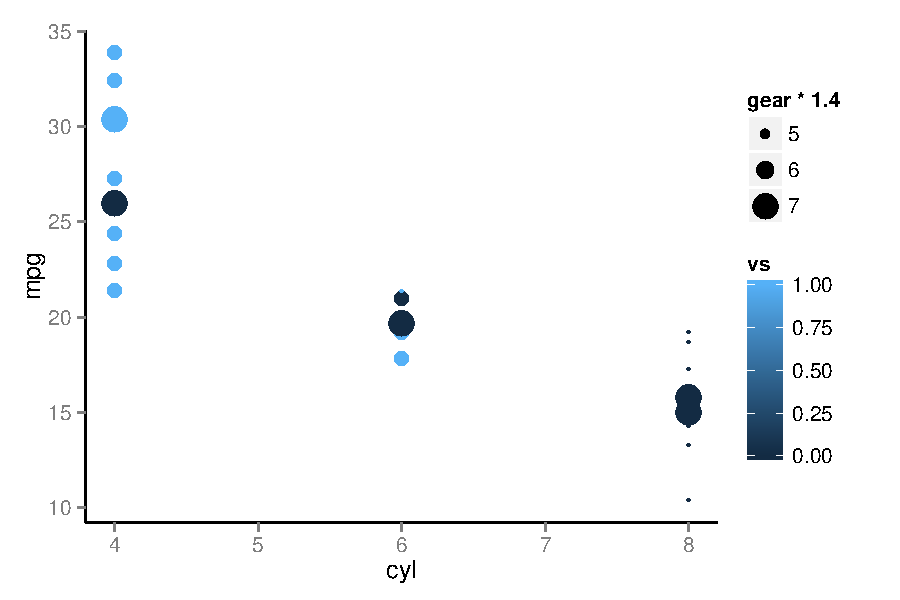
\includegraphics[width=.75\linewidth]{figure/boring-random} 

\end{knitrout}

\end{frame}

\begin{frame}[fragile]
Now we can vary the gear size.
\begin{knitrout}\footnotesize
\definecolor{shadecolor}{rgb}{0.969, 0.969, 0.969}\color{fgcolor}\begin{kframe}
\begin{alltt}
\hlfunctioncall{ggplot}(mtcars, \hlfunctioncall{aes}(cyl, mpg, color = vs)) +
\hlfunctioncall{geom_point}(\hlfunctioncall{aes}(size = gear * 1.4))
\end{alltt}
\end{kframe}
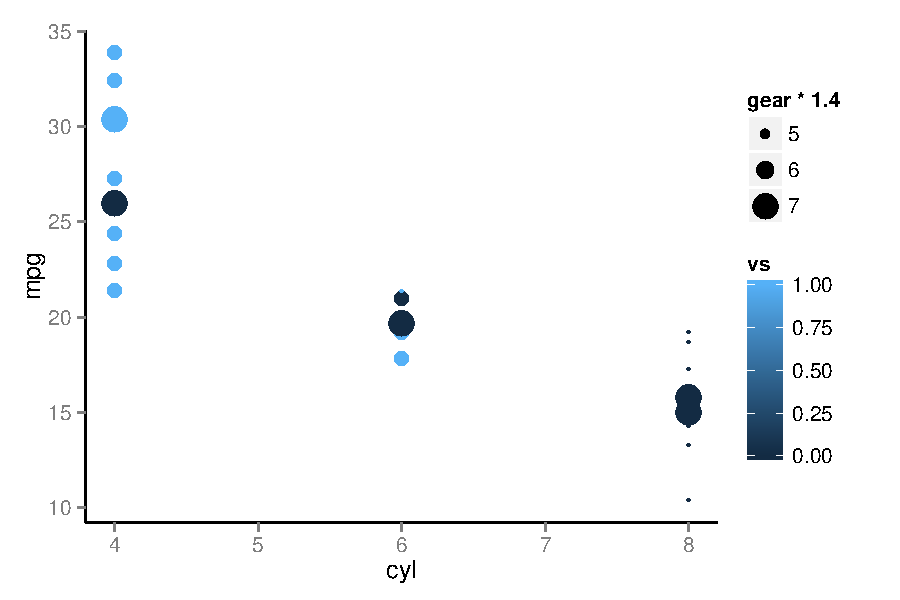
\includegraphics[width=.75\linewidth]{figure/boring-randomb_} 

\end{knitrout}

\end{frame}



\begin{frame}[fragile]
The first element of \texttt{x} is 1. Boring boxplots
and histograms recorded by the PDF device:

\begin{knitrout}\footnotesize
\definecolor{shadecolor}{rgb}{0.969, 0.969, 0.969}\color{fgcolor}\begin{kframe}
\begin{alltt}
x <- \hlfunctioncall{rnorm}(100)
y <- 1
\end{alltt}
\end{kframe}
\end{knitrout}

\end{frame}

\begin{frame}[fragile]
The first element of \texttt{x} is -0.6809. Boring boxplots
and histograms recorded by the PDF device:

\begin{knitrout}\footnotesize
\definecolor{shadecolor}{rgb}{0.969, 0.969, 0.969}\color{fgcolor}\begin{kframe}
\begin{alltt}
\hlfunctioncall{ggplot}(data, \hlfunctioncall{aes}(x, y)) + \hlfunctioncall{geom_point}(size = 4)
\end{alltt}
\end{kframe}
\end{knitrout}


\begin{knitrout}\footnotesize
\definecolor{shadecolor}{rgb}{0.969, 0.969, 0.969}\color{fgcolor}\begin{kframe}
\begin{alltt}
\hlfunctioncall{ggplot}(data, \hlfunctioncall{aes}(x, y)) + \hlfunctioncall{geom_point}(size = 4)
\end{alltt}
\end{kframe}
\end{knitrout}


\begin{knitrout}\footnotesize
\definecolor{shadecolor}{rgb}{0.969, 0.969, 0.969}\color{fgcolor}\begin{kframe}
\begin{alltt}
\hlfunctioncall{ggplot}(data, \hlfunctioncall{aes}(x, y)) + \hlfunctioncall{geom_point}(size = 4)
\end{alltt}
\end{kframe}
\end{knitrout}

\end{frame}

\begin{frame}[fragile]
The first element of \texttt{x} is -0.6809. Boring boxplots
and histograms recorded by the PDF device:

\begin{knitrout}\footnotesize
\definecolor{shadecolor}{rgb}{0.969, 0.969, 0.969}\color{fgcolor}
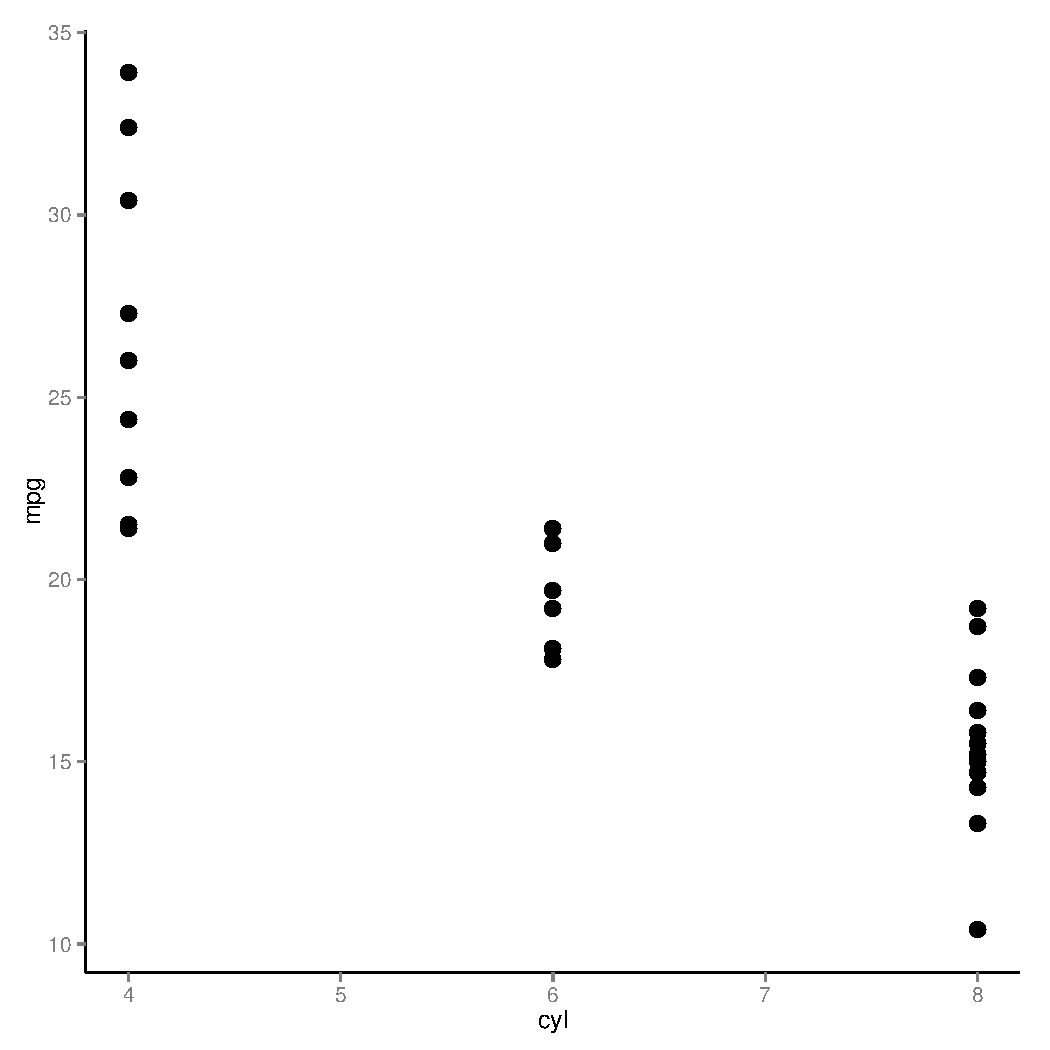
\includegraphics[width=.75\linewidth]{figure/tempec} 

\end{knitrout}


\end{frame}



\end{document}
